
\documentclass[12pt]{article}
\usepackage{pgf}
\usepackage{pgflibraryshapes}
\usepackage{tikz}

\begin{document}

\thispagestyle{empty}
\setlength{\fboxrule}{0.01pt}
\setlength{\fboxsep}{4pt}

\fbox{

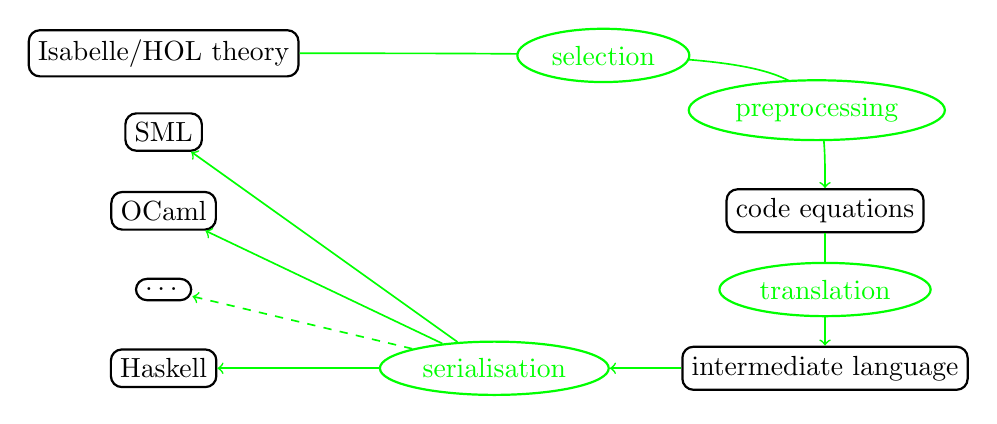
\begin{tikzpicture}[x = 4.2cm, y = 1cm]
  \tikzstyle entity=[rounded corners, draw, thick, color = black, fill = white];
  \tikzstyle process=[ellipse, draw, thick, color = green, fill = white];
  \tikzstyle process_arrow=[->, semithick, color = green];
  \node (HOL) at (0, 4) [style=entity] {Isabelle/HOL theory};
  \node (eqn) at (2, 2) [style=entity] {code equations};
  \node (iml) at (2, 0) [style=entity] {intermediate language};
  \node (seri) at (1, 0) [style=process] {serialisation};
  \node (SML) at (0, 3) [style=entity] {SML};
  \node (OCaml) at (0, 2) [style=entity] {OCaml};
  \node (further) at (0, 1) [style=entity] {\ldots};
  \node (Haskell) at (0, 0) [style=entity] {Haskell};
  \draw [style=process_arrow] (HOL) .. controls (2, 4) ..
    node [style=process, near start] {selection}
    node [style=process, near end] {preprocessing}
    (eqn);
  \draw [style=process_arrow] (eqn) -- node (transl) [style=process] {translation} (iml);
  \draw [style=process_arrow] (iml) -- (seri);
  \draw [style=process_arrow] (seri) -- (SML);
  \draw [style=process_arrow] (seri) -- (OCaml);
  \draw [style=process_arrow, dashed] (seri) -- (further);
  \draw [style=process_arrow] (seri) -- (Haskell);
\end{tikzpicture}

}

\end{document}
